\documentclass[tikz]{standalone}
\usepackage{pgfplots}
\usepgfplotslibrary{groupplots}
\pgfplotsset{compat=1.18}
\definecolor{utnblue}{RGB}{0, 102, 204}

\begin{document}
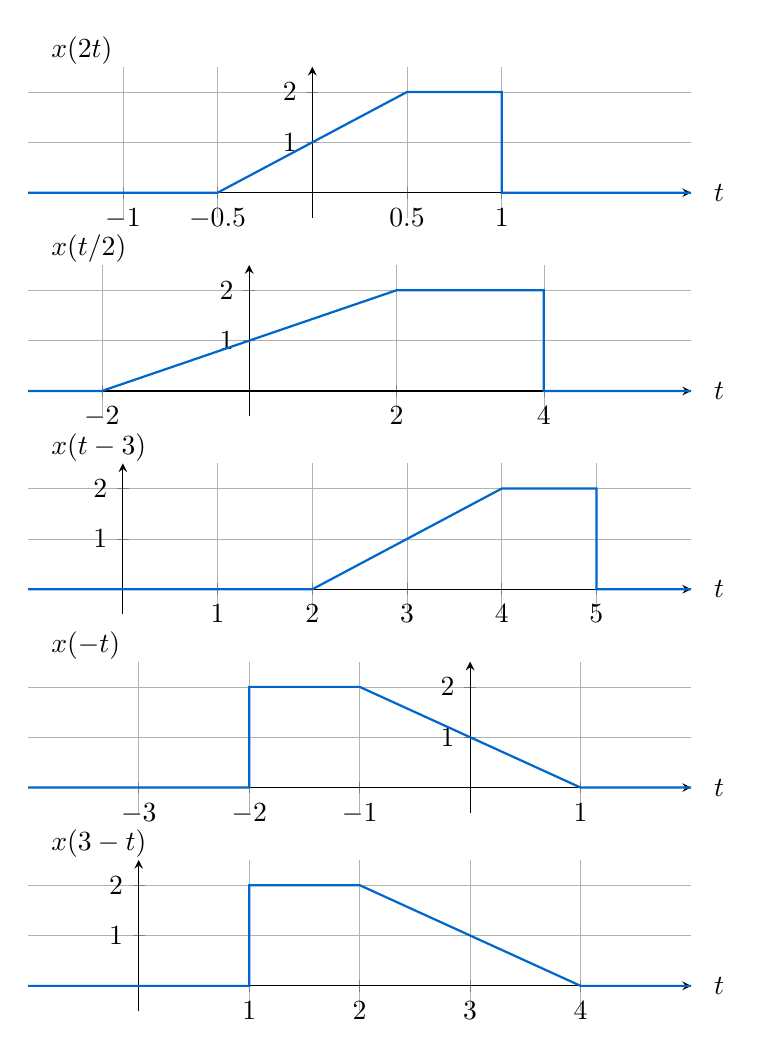
\begin{tikzpicture}
    \begin{groupplot}[
        group style={
            group size=1 by 5,
            vertical sep=0.6cm,
        },
        width=10cm,
        height=3.5cm,
        axis lines=middle,
        grid=both,
        grid style={line width=.1pt, draw=gray!40},
        major grid style={line width=.2pt,draw=gray!60},
        every axis plot/.append style={thick},
        every axis x label/.append style={at={(ticklabel* cs:1.02)}, anchor=west},
        every axis y label/.append style={at={(rel axis cs:0.02, 0.95)}, anchor=south west, rotate=0},
    ]
    
    % (a) x(2t): soporte [-1/2, 1], rampa 2t+1 en [-1/2, 1/2], constante 2 en [1/2, 1]
    \nextgroupplot[
        xmin=-1.5, xmax=2, ymin=-0.5, ymax=2.5,
        xtick={-1,-0.5,0,0.5,1}, ytick={0,1,2},
        ylabel={$x(2t)$}, xlabel={$t$},
    ]
    \addplot[utnblue] coordinates {(-1.5,0) (-0.5,0) (0.5,2) (1,2) (1,0) (2,0)};
    
    % (b) x(t/2): soporte [-2, 4], rampa t/2+1 en [-2, 2], constante 2 en [2, 4]
    \nextgroupplot[
        xmin=-3, xmax=6, ymin=-0.5, ymax=2.5,
        xtick={-2,0,2,4}, ytick={0,1,2},
        ylabel={$x(t/2)$}, xlabel={$t$},
    ]
    \addplot[utnblue] coordinates {(-3,0) (-2,0) (2,2) (4,2) (4,0) (6,0)};
    
    % (c) x(t-3): soporte [2, 5], rampa t-2 en [2, 4], constante 2 en [4, 5]
    \nextgroupplot[
        xmin=-1, xmax=6, ymin=-0.5, ymax=2.5,
        xtick={0,1,2,3,4,5}, ytick={0,1,2},
        ylabel={$x(t-3)$}, xlabel={$t$},
    ]
    \addplot[utnblue] coordinates {(-1,0) (2,0) (4,2) (5,2) (5,0) (6,0)};
    
    % (d) x(-t): 0 para t<-2, salto a 2 en t=-2, constante 2 en [-2,-1],
    %     rampa 1-t en [-1,1] (de 2 a 0), 0 para t>1
    \nextgroupplot[
        xmin=-4, xmax=2, ymin=-0.5, ymax=2.5,
        xtick={-3,-2,-1,0,1}, ytick={0,1,2},
        ylabel={$x(-t)$}, xlabel={$t$},
    ]
    \addplot[utnblue] coordinates {(-4,0) (-2,0) (-2,2) (-1,2) (1,0) (2,0)};
    
    % (e) x(3-t): 0 para t<1, salto a 2 en t=1, constante 2 en [1,2],
    %     rampa 4-t en [2,4] (de 2 a 0), 0 para t>4
    \nextgroupplot[
        xmin=-1, xmax=5, ymin=-0.5, ymax=2.5,
        xtick={0,1,2,3,4}, ytick={0,1,2},
        ylabel={$x(3-t)$}, xlabel={$t$},
    ]
    \addplot[utnblue] coordinates {(-1,0) (1,0) (1,2) (2,2) (4,0) (5,0)};
    
    \end{groupplot}
\end{tikzpicture}
\end{document}
